\section{Terrain-Vehicle Model Validation}
Experimental data for a Caterpillar/AGCO MT865 tractor were collected in Antarctic conditions using the vehicle's J1939 Controller Area Network (CAN), an 18x 5 Hz Garmin GPS, and the same analog load pin circled in red in Fig. \ref{fig:Tractor_Load_Pin} to measure the drawbar force. Data were acquired while the vehicle towed a sled containing $\sim$80,000kg of fuel bladders. The measured values include $\Omega_E$, $\Pi_I$, $g_{GR}$, $\dot\varphi_L$  and $\dot\varphi_R$, $v_T$, and $DB$ to denote the engine speed, engine percent torque demand or throttle input, gear ratio number, left and right driver speeds, tractor speed and drawbar load. These values allow longitudinal motion validation of the model presented in section \ref{s:Rigid_Body_Dynamics}. The equations of motion for longitudinal motion reduce to
\begin{equation}\label{eq:GBSD_MV}
    \dot v_T = \frac{F_L + F_R - R_L - R_R - DB}{m_T}
\end{equation}
\begin{equation}\label{eq:WBSDL_MV}
    \ddot\varphi_L = \frac{(\tau_L - F_L - \zeta\dot\varphi_L)}{J_S}
\end{equation}
\begin{equation}\label{eq:WBSDR_MV}
    \ddot\varphi_R = \frac{(\tau_R - F_R - \zeta\dot\varphi_R)}{J_S}
\end{equation}
% ---------------------- Paragraph --------------------------
 The result is that the lateral track resistance forces are null and the higher order terms are eliminated. In addition, data where the tractor-sled system is operating at steady-state or an equilibrium point is used to approximate terrain parameters. In this operating condition eq.'s \ref{eq:GBSD_MV}-\ref{eq:WBSDR_MV} become eq.'s \ref{eq:GBSD_MV_SS}-\ref{eq:WBSDR_MV_SS}.
\begin{equation}\label{eq:GBSD_MV_SS}
    0 = F_L + F_R - R_L - R_R - DB
\end{equation}
\begin{equation}\label{eq:WBSDL_MV_SS}
    0 = \tau_L - F_L - \zeta\dot\varphi_L
\end{equation}
\begin{equation}\label{eq:WBSDR_MV_SS}
    0 = \tau_R - F_R - \zeta\dot\varphi_R
\end{equation}
In eq. \ref{eq:GBSD_MV_SS}, the drawbar load $DB$ is treated as a model input since it is directly measured and the driver torques $\tau_L$ and $\tau_R$ in eq.'s \ref{eq:WBSDL_MV_SS} and \ref{eq:WBSDR_MV_SS} as known since detailed powertrain, truth data is provided by AGCO. $F_L$ and $F_R$ are then approximately solved for and matched with corresponding slip values. Using these values, track resistance forces $R_L$ and $R_R$ can be estimated. The values of the tractive forces are used for approximating the terrain parameters of cohesion, $c$, the friction angle, $\Phi$, and the shear deformation modulus $K$ while the track resistance forces are left as an estimated constant value. The three parameters $c$, $\Phi$ and $K$ determine the shape of the force-slip curves shown in Fig. \ref{fig:force_slip_curve}. In Fig. \ref{fig:force_slip_curve_vary_K} it can be seen that the shear deformation modulus has a noticeable effect on the slope of the tractive effort in the linear region at low slip values. In Fig. \ref{fig:force_slip_curve_vary_cphi}, the increases in cohesion and friction angle lead to increases in the maximum shear stress,  that can be loaded on the terrain. This has noticeable effects on the tractive effort developed at higher slips. The effects of these parameters in each region are accounted for when estimating terrain parameters and since the vehicle operated at lower slip values during data collection, there is a higher confidence in the proposed $K$ value relative to $c$ and $\Phi$.

The model is validated by simulation where a tractor starts from rest or zero initial conditions at $t = 0$ using the inputs of the driver during data collection of $\Pi_I$ and $g_GR$.
\begin{figure}[hb]
\begin{subfigure}{0.5\textwidth}
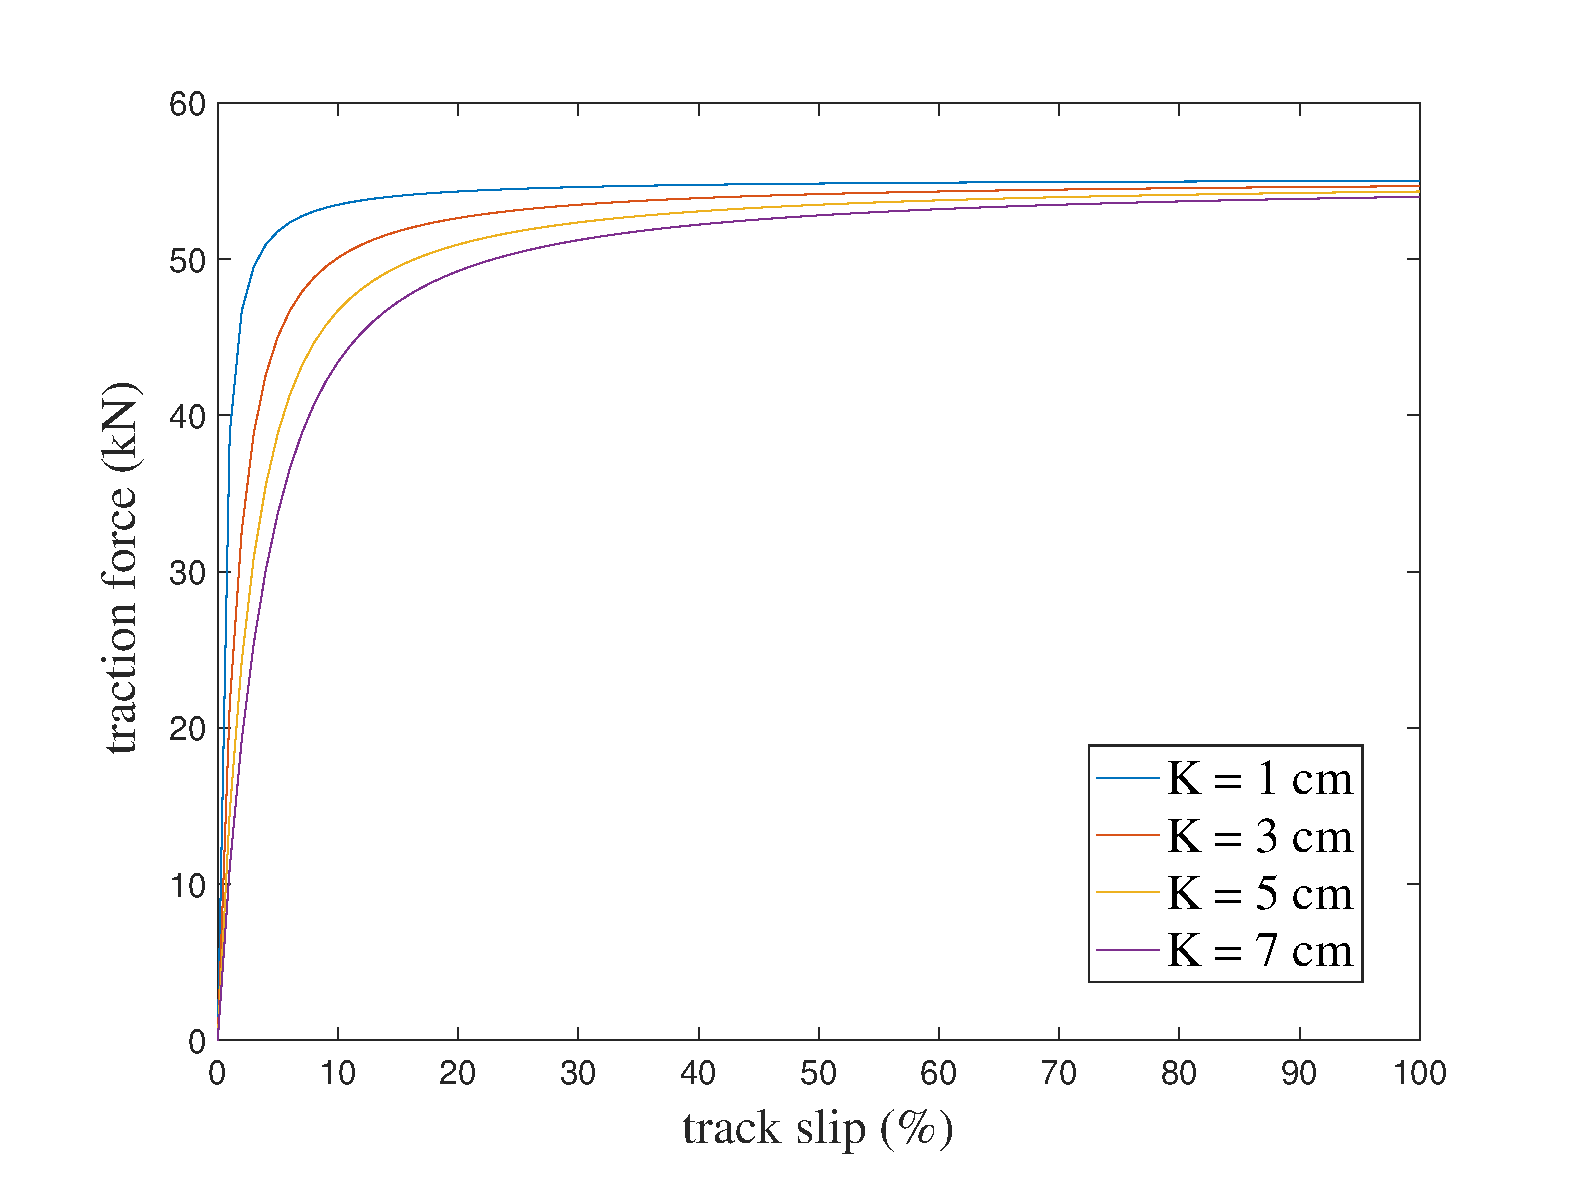
\includegraphics[width = 7.5 cm, height = 6 cm]{force_slip_curve_vary_K}
\caption{}
\label{fig:force_slip_curve_vary_K}
\end{subfigure}
\begin{subfigure}{0.525\textwidth}
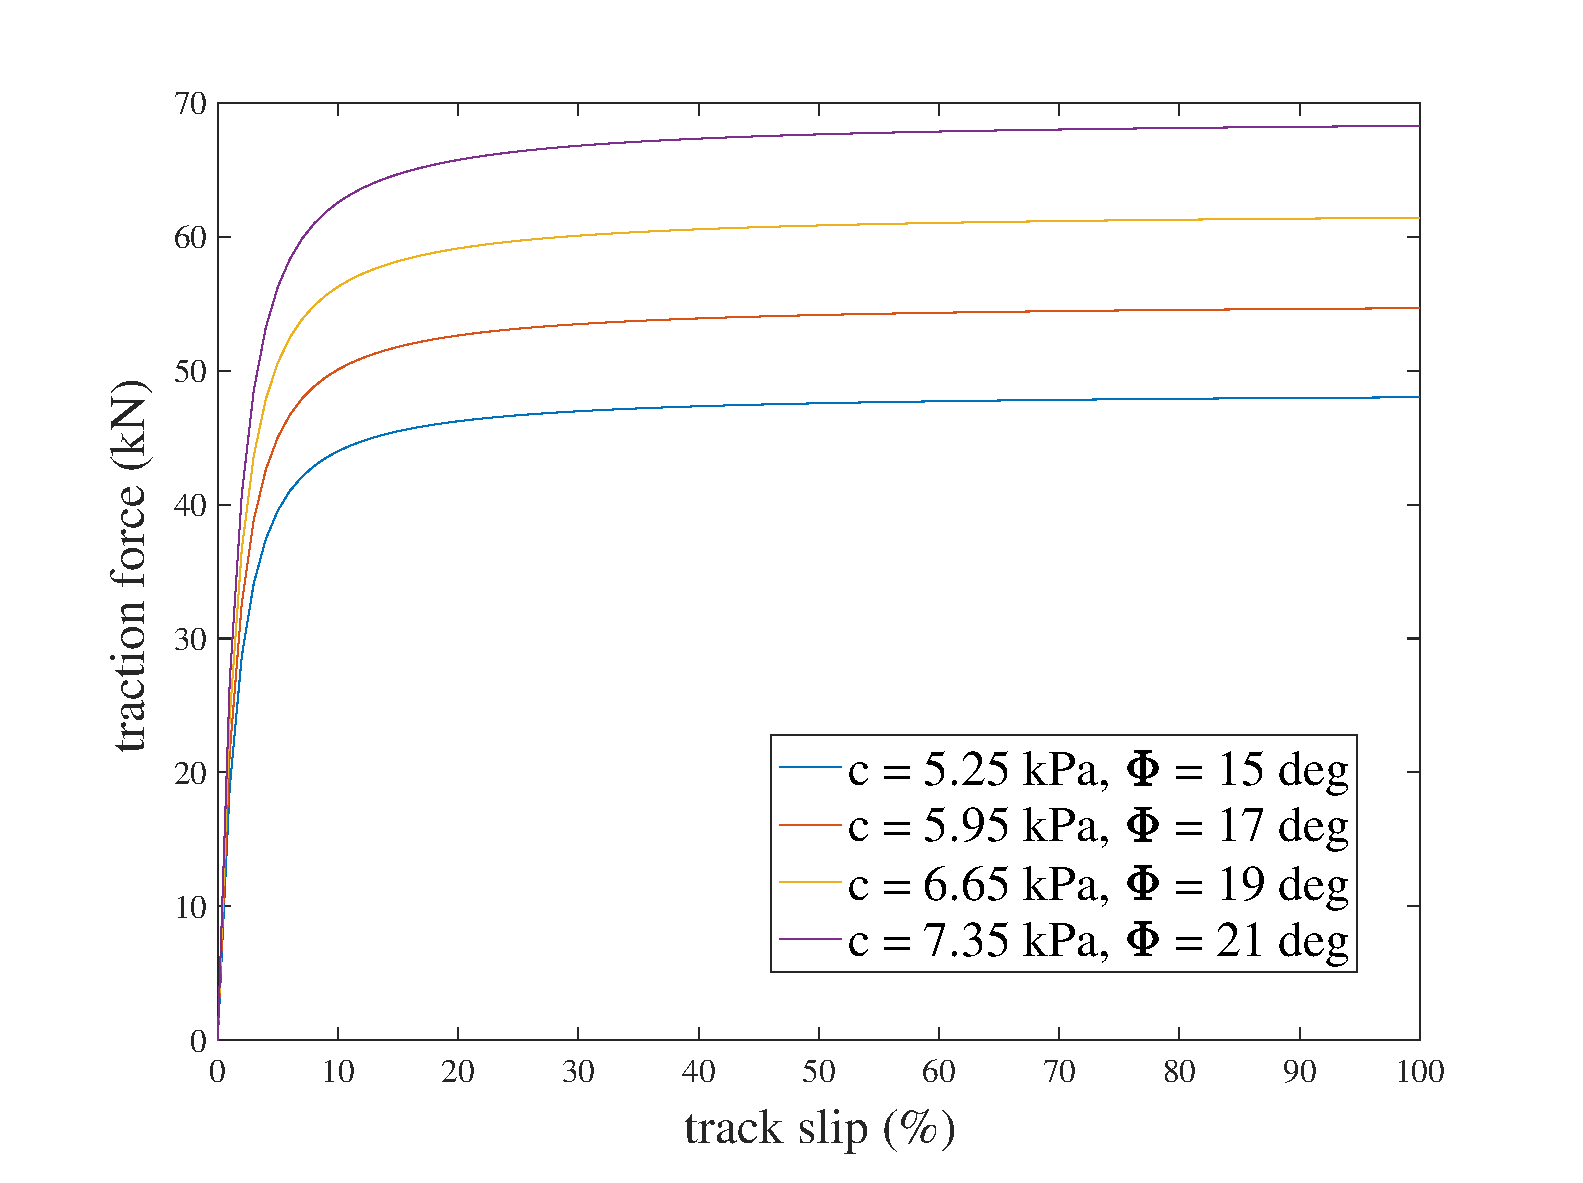
\includegraphics[width = 7.5 cm, height = 6cm]{force_slip_curve_vary_cphi}
\caption{}
\label{fig:force_slip_curve_vary_cphi}
\end{subfigure}
\caption{Plots of force-slip curves using Wong terramechanics theory from Eq. \ref{eq:tractionForce}. (a) Force-slip curves for varying values of the shear deformation modulus, K (cm).  (b) Force-slip curve with varying of cohesion, $c$ (kPa), and friction angle $\Phi$ (deg).}
\label{fig:force_slip_curve}
\end{figure}
Other inputs to the model for simulation are the estimated terrain parameters of $K=2$ cm, $c = 10$ kPa, and $\Phi=19$ degrees and the total resistance $R_{total} = R_L + R_R + DB$. In Fig. \ref{fig:Model_Validation_Plot_Sim}, model predictions or simulation results are plotted against experimental data as blue and black lines respectively for four minutes of data during which the tractors starts from rest and ramps up to a steady velocity while shifting through gears. Measured and simulated responses for $v_T$, $\dot\varphi_L$ and $\dot\varphi_R$, $i_L$ and $i_R$, $\Omega_E$ and $P_E$ are provided in Fig. \ref{fig:Model_Validation_Plot_Sim}. 
\begin{figure}[hb]
    \centering
    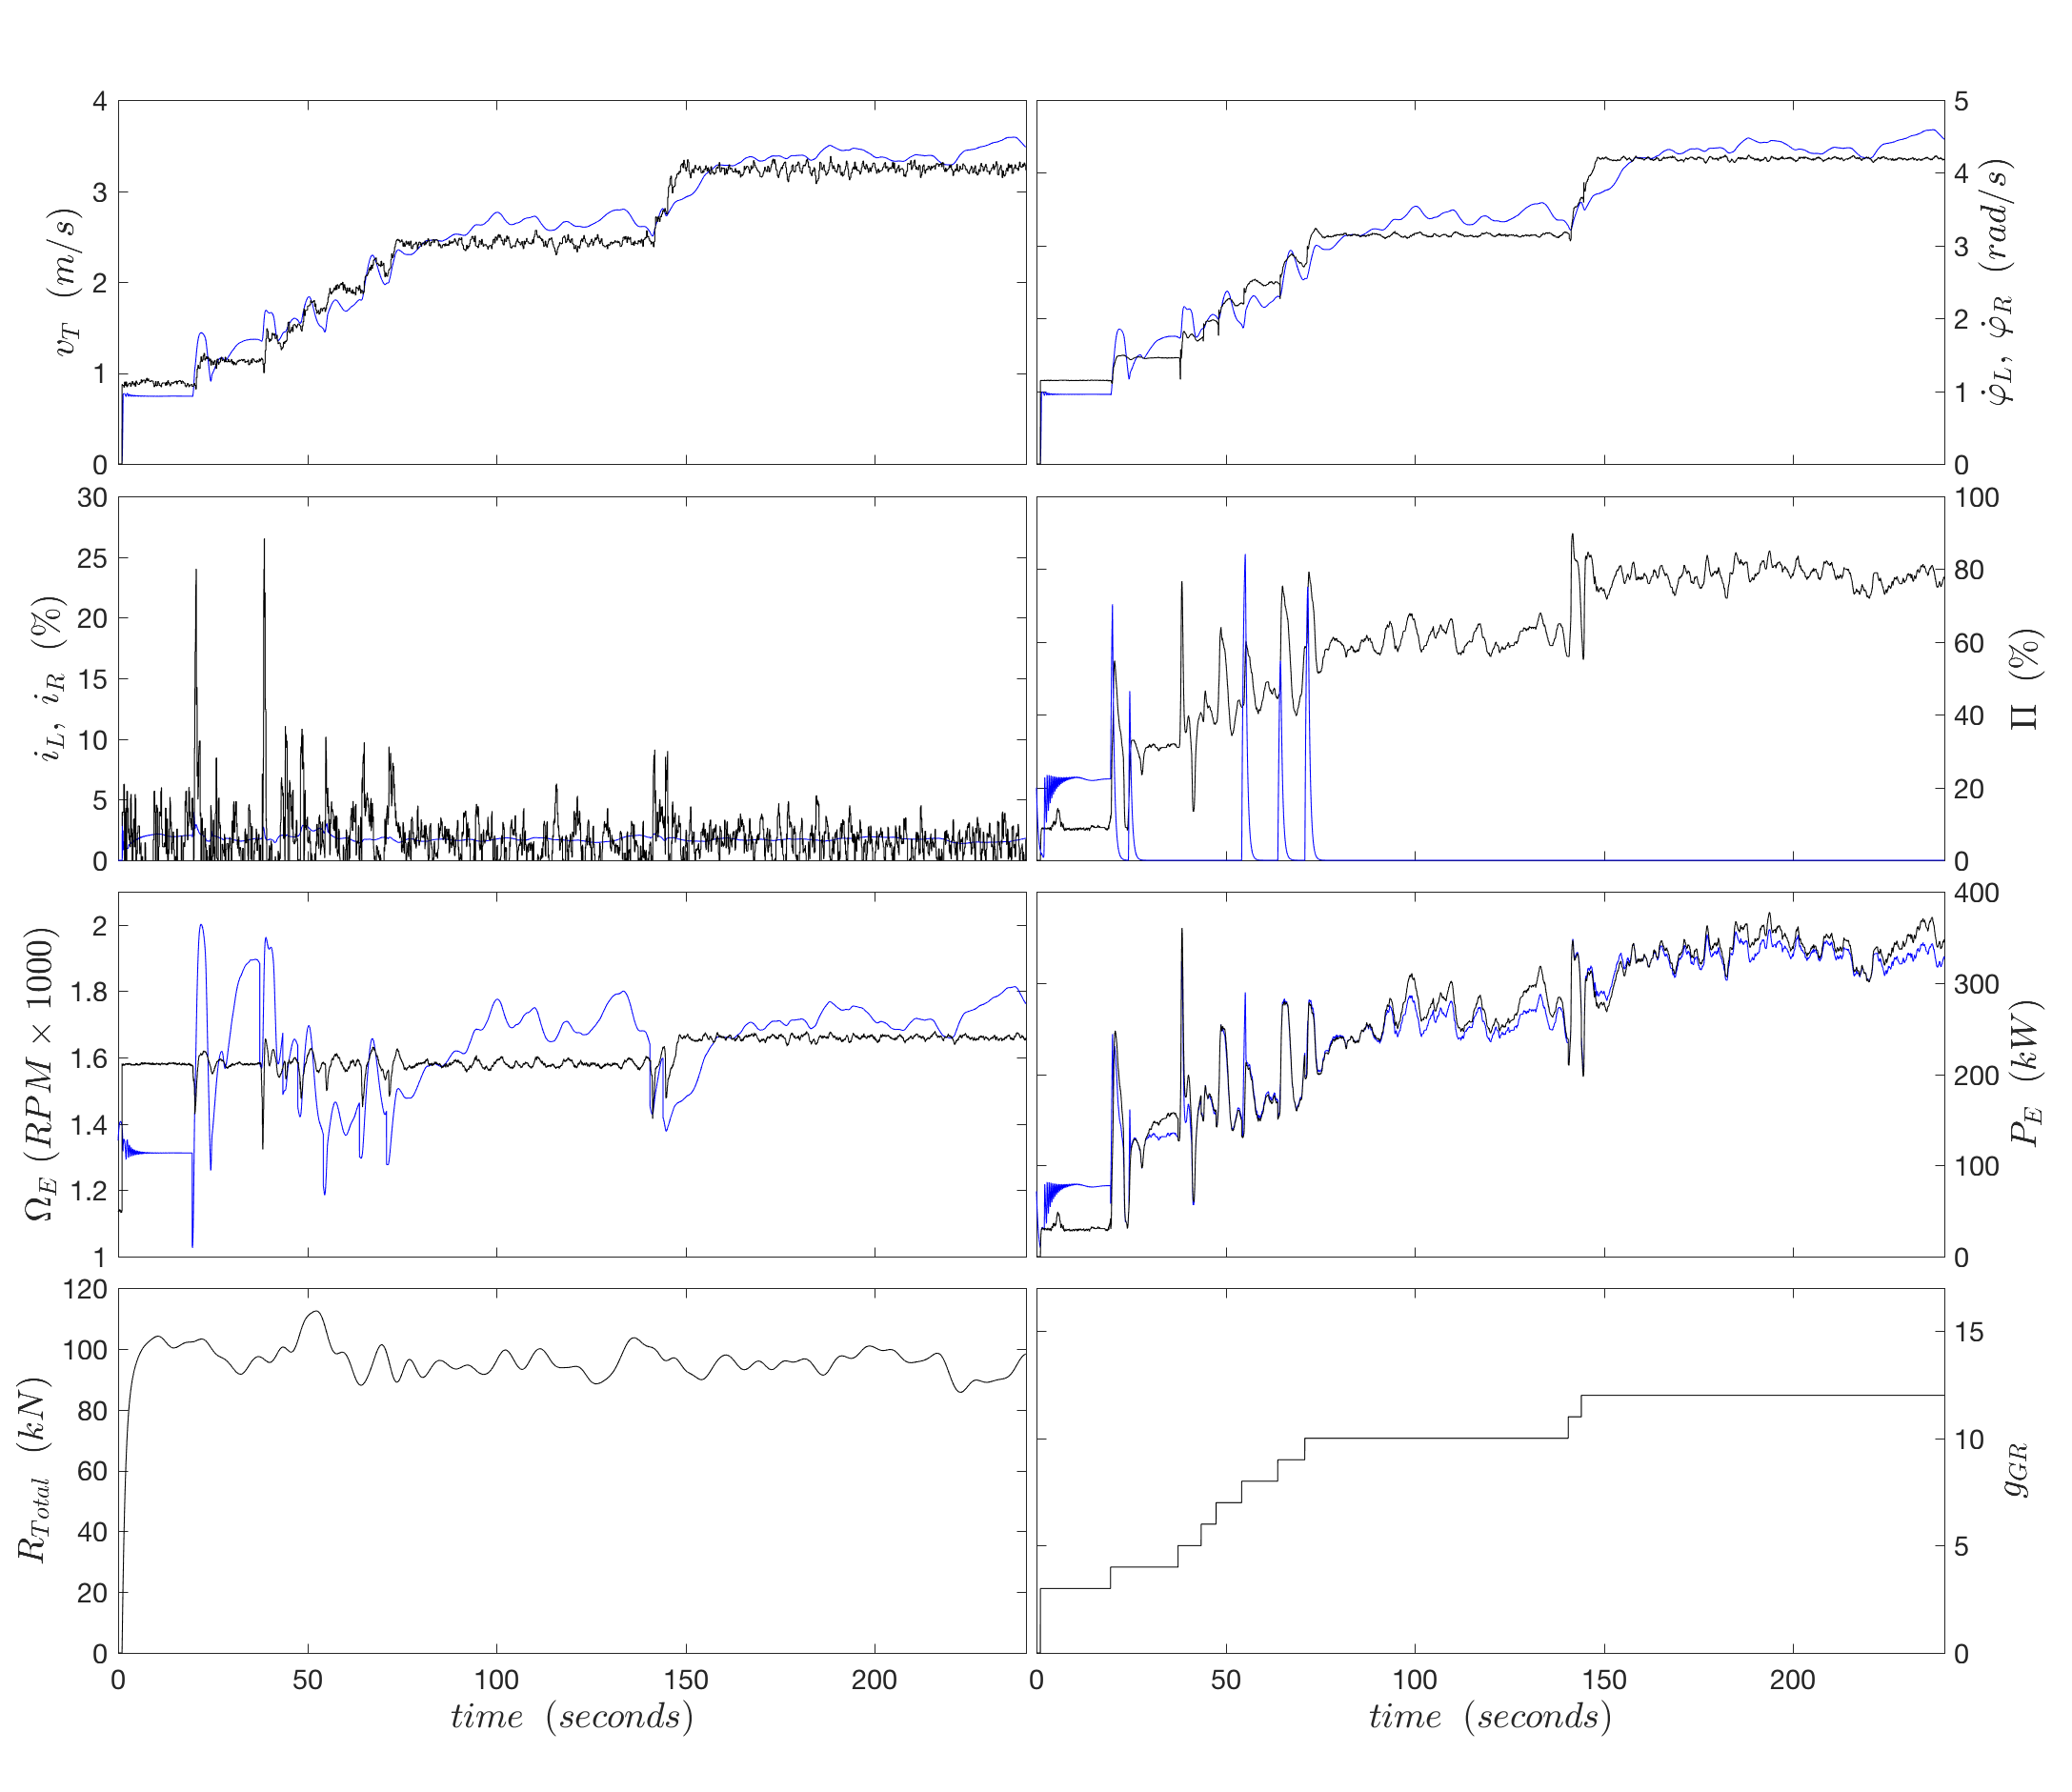
\includegraphics[width = 6in]{Model_Validation_Plot_Sim}
    \caption{$v_T$, $\dot\varphi_L$, $\dot\varphi_R$, $i_L$, $i_R$, $\Omega_E$, and $P_E$ are plotted as solid and dashed lines corresponding to model predictions and experimental data respectively. Inputs to the model are $\Pi$, $g_{GR}$, and $R_{Total} = R_L + R_R + DB$ plotted as dashed lines. The solid line on the $\Pi$ plot is the overriding controller, $\Pi_C$ to prevent engine stalling. Values for track resistance forces are made from estimated unmeasured terrain parameters and are assumed constant}
    \label{fig:Model_Validation_Plot_Sim}
\end{figure}
The blue line on the $\Pi$ plot is the output of an overriding engine controller, $\Pi_C$ to prevent stalling. The equations for $\Pi$ and $\Pi_C$ are from \cite{MathWorks2015GenericEngine}.
\begin{equation}
    \Pi = \max(\Pi_I,\Pi_C)
\end{equation}
\begin{equation}
    \dot\Pi_C = \frac{1}{\delta_E}\Bigg( \Big(0.5 - 0.5\tanh\frac{\omega_E-\omega_I}{\omega_T}\Big) - \Pi_C  \Bigg)
\end{equation}
The controller overrides the driver input for the first 25-30 seconds in 3rd gear and at several other points during gear shifts. This highlights the model's simplifying assumptions as presented which assume constant track resistance forces. It is plausible that different terrain was encountered during the beginning of data collection and this assumption does not hold for all time. In addition, it is postulated that the discrepancies during gear shifts can be accounted for by the use of oversimplified dynamics that do not account for control mechanisms. However, predictions at all other points prove to be accurate and show that the model sufficiently couples the powertrain with the vehicle-terrain dynamics.

